\documentclass{ctexart}
\usepackage{geometry}
\usepackage{diagbox}
\usepackage{graphicx}
\usepackage{subfigure}
\usepackage{amsmath}
\usepackage{amssymb}
\usepackage{indentfirst}
\usepackage{xfrac}
\usepackage{color}
\usepackage[table]{xcolor}
\usepackage{multirow}
\usepackage{titlesec}
\usepackage{bm}
\usepackage{caption}
\title{UP主粉丝数的影响因素分析}
\author{CDA小组}
\date{}
\begin{document}
\maketitle
\begin{abstract}
    这里是摘要
\end{abstract}
\section{背景介绍}
Bilibili视频网站(下文简称B站)在近年愈发受到年轻人的欢迎,数量庞大的UP主群体为B站的视频生态的多样性做出了
非常大的贡献。在庞大的UP主群体之下,UP主的粉丝数也有显著的差异。本研究旨在通过研究各种影响因素与UP主的粉丝
数量的分层不同带来的影响。\\
\indent 本次研究的数据来源于ifans网站,网站上提供了粉丝量、最近更新时间、分区、视频数、
充电数、近8篇平均视频投币数、近8篇平均视频弹幕数、近8篇平均视频收藏数、近8篇平均视频点赞数、
近8篇平均视频播放数、近8篇平均视频评论数、近8篇平均视频分享数数据、性别数据,本研究将所有变量均放入模型中进行研究,
同时研究是否能够有减少变量的方法。本研究凭借网站上的粉丝数量分区,
将粉丝量的分区分为“<10万”,“10万~50万”,“50万~100万”,“>100万”四个分区,作为后续分类型数据分析的基础。\\
\indent 由于不同分区的UP主人数差异较大,本研究采用回溯性研究方法,即在四个粉丝量的分区分别抽取250个UP主的数据
进行研究分析。
\section{数据预处理}
由于每个变量的单位相差较大,为了避免单位造成的影响,本研究将所有非分类型数据进行归一化处理。
由于选择的解释变量均为非负数据,为保持这一性质,采用以下的归一化方法。
\begin{equation}
    \tilde{x} = \frac{x-\alpha}{\beta - \alpha}
\end{equation}
其中$\alpha$,$\beta$分别为本解释变量中的最大值与最小值。
\section{探索性数据分析}
\subsection{数据可视化}
首先,作出各类数据之间相关系数的热度图:
\begin{figure}[htbp]
    \centering
    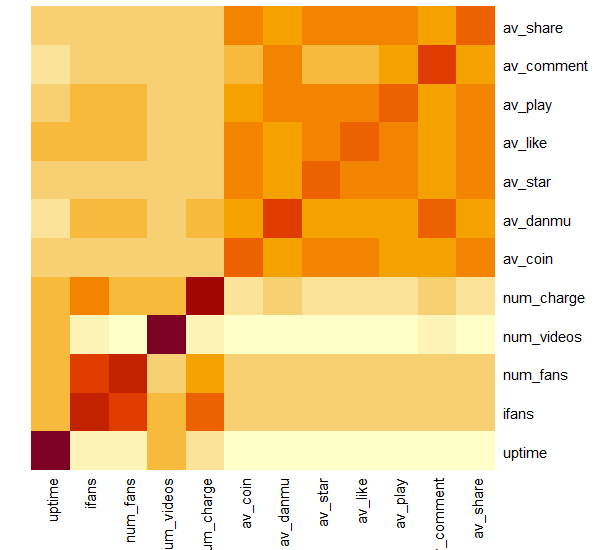
\includegraphics[width=0.60\textwidth]{EDA/Heatmap.png}
    \caption{Heatmap for Correlation}
\end{figure}
\end{document}